\documentclass[]{report}
\usepackage{graphicx}
\usepackage{mathtools}
\usepackage{listings}
\usepackage{fancyvrb}
\fvset{tabsize=2}
\lstset{language = Python, numbers = left, stepnumber = 1,literate={\ \ }{{\ }}1,tabsize =2}
% Title Page
\title{Using Blade Element Momentum Theory for Propeller Analysis}
\author{Nicholas McCaw}


\begin{document}
\maketitle
\begin{abstract}
\end{abstract}

\chapter{Introduction}
This report outlines the work completed during the 1st year of the EngD program. This chapter will give an outline of the content of the report as well as the motivation for doing the project. 

The second chapter of the report gives a brief overview of the literature which has been reviewed, the third chapter details the background theory of blade element momentum theory, Timoshenko beam theory and finite element analysis. The fourth chapter will discuss the code developed using these techniques and some preliminary results obtained.
\\
\\
Propellers are the most widely used form of propulsion for marine vehicles. It is desired for the noise to be reduced. This is to  increase efficiency and to reduce the environmental impact. 

To lessen the noise of the propeller it is vital to reduce vibration. Vibration is caused by the fluid interacting with the structure. The geometry of the propeller blade causes a pressure difference between its two surfaces. This pressure difference causes a force in the direction toward the low pressure side, normal to the surface of the blade. This phenomena is used to produce thrust. 
\\
However the load on the propeller blade causes the blade to deform. The changed blade shape then causes the load produced to be changed which, in turn, causes the shape of the propeller blade to change. This is the fundamentals of hydroelastics.
\\
A computationally inexpensive way to obtain the propeller blade loads is to use blade element momentum theory. To obtain blade deformations the blade is treated as a simple 1D Timoshenko Beam and Timoshenko beam theory is used along side 1D finite element analysis. Both these techniques will be discussed in more detail in chapter 3. Finally the code produced will be discussed in chapter 4

\chapter{Literature Review}
Firstly the International Towing Tank Conference (ITTC) (CITATION) notes where reviewed. This was mainly to review the state of the art marine technology.

The ITTC propulsion committee was reviewed. This detailed the most up to date propulsion technologies and current research trends. Furthermore it detailed areas where more research was required. 
The first item of new technology was counter-rotating propellers which have the advantage over single propellers due to having two propellers sharing the propulsive force hence a reduction is rotation speed is obtained(INSERT CITATION). This is beneficial as the reduced reduction speed will result in reduced vibration and hence noise. 
Flexible blade propulsors are also of high interest to researchers. This is because having fully composite propeller blades offer significant weight saving (TTC Citation). Furthermore composites can be passively tailored during loading thus improving performance. This is of particular interest to researchers as the examples of propellers made from composite materials have been shown to have a higher efficiency (BLACK 2011) and cavitation speed (Kane 2001). 
\\
This area of hydroelastics is of interest to the project therefore the paper by Young (YOUNG 2006) was read further. This paper described the numerical model and solution procedure for modelling the hydroelastic response of composite marine propellers. The numerical model was a 3D boundary element method with the total flow velocity composed of inflow velocity and a propeller induced perturbation. The solution procedure involved computing the hydrodynamic added mass and damping. The pressure is calculated using the boundary element method. The deformations can then be calculated and applied to the new blade geometry. This process is repeated until the solution converges. A similar procedure is implemented in the code described in chapter 4. 

The ITTC proceeding then went on to describe the need for research and development. The areas where:
\begin{enumerate}
	\item Model and fullscale measurements of propulsors in off-design conditions
	\item Full scale measurements of ship propulsive gain due to use of energy saving devices.
	\item Propulsive performances on composite propeller at full scale and model scale with measurement of blade deformation and torque.
	\item full-scale measurement on hybrid contra-rotating shaft pod propulsors.
	\item CFD simulation on the effect of varying Reynolds numnber on the performance of blade sections.
	\item full scale measurement of waterjet inlet flow velocity fields.
\end{enumerate}


Points 3. and 5. relate closely to the project undertaken this year.
\\

The ITTC proceedings had a large section based on energy saving devices such as: wake equalizing ducts and pre-swirl stators. This section was read however it was deemed out of the scope of this project. 

Other new technologies where described in the proceedings including: surface piercing propellers (HIMEI ET AL 2013), High speed vehicles and contracted and loaded tip propellers. 
\\
After this review it was decided to focus on the propeller blade deformation and CFD of Reynolds number effects.
\
To model the Reynolds number effect using CFD a CFD package must be used. It was decided that open source software would be desirable hence OpenFOAM was used.

\section{OpenFOAM Tutorials}

I was decided that the OpenFOAM would be the CFD software of choice due to the open source nature. This means that the software can be easily changed to suit the needs of the user. Also the software is free making it cheaply used on many cores.

This sub-section will describe the tutorials undertaken using OpenFOAM.The first tutorials objective is to introduce the meshing and simulation of a simple test case. The test case used in this example is a lid-driven cavity flow. 
Firstly the mesh is created. This is done by defining the vertices of the block the user wishes to populate with cells. The number of cells are then defined in the x,y and z directions with any grading defined along each direction. For the initial case a uniform grid is created. Finally the wall boundary conditions are defined with the sides and bottom set to fixed and the top wall set to moving. The mesh is then created using the 'blockMesh' command. 
\
Once the mesh has been generated the fluid flow conditions can be analysed. There are two files for this test case: a pressure file and a velocity file. Within the pressure file the dimensions of the pressure field (i.e kinematic pressue), the kinematic pressure field value (zero for the initial condition) and the wall boundary conditions are all defined. The fixed walls and moving wall are set to have a normal gradient of pressure of zero. Similar conditions are set in the velocity field file. The kinematic viscosity $ \nu$ was then set to fix the Reynolds number.
\ 
The time-step must then be selected such that the simulation is stable. When running 'icoFOAM' stability and accuracy are ensured by keeping the Courant number less than one throughout the domain. This is done using the equation: 
\begin{equation}
Co = \frac{\delta t |U| }{\delta x}
\label{eq:courant}
\end{equation}

When the grid is uniform i.e $\delta x$ is constant this is a simple condition to meet. However in non-uniform grids this becomes slightly more difficult. 
 
The appropriate timestep $\delta t$ can therefore be calculated using equation \ref{eq:courant}. 
\\
The finite volume discretisation solver can then be specified. The mesh is then viewed in ParaView to ensure it has been generated correctly. The simulation is then run using icoFOAM. The residuals and maximum Courant numbers are displayed as the simulation is running.
\
Once the simulation is complete the pressures can be plotted as shown in \ref{fig:cavity_pressure}

\begin{figure}[h]
	\centering
	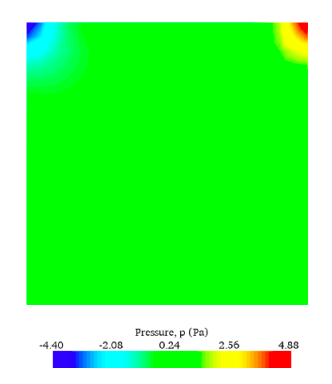
\includegraphics[scale=0.5]{cavity_pressure}
	\caption{Pressures in Cavity test case}
	\label{fig:cavity_pressure}
\end{figure}

It can be seen from \ref{fig:cavity_pressure} that there is a low pressure at the top left corner of the cavity with higher pressure at the top right corner. This is as expected because the flow is moving from left to right within the cavity. The flow features can be seen in greater detail if the velocity vectors are shown as in figure \ref{fig:cavity_vector}. 
\newpage
\begin{figure}[h]
	\centering
	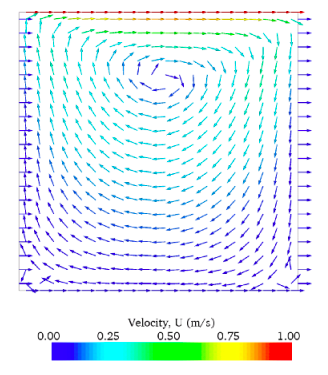
\includegraphics[scale=0.5]{cavity_vector.png}
	\caption{Vectors in Cavity test case}
	\label{fig:cavity_vector}
\end{figure}
\
Here it is seen that a small vortex has been created within the cavity. However it is noted that the resolution of the vectors are not good. It is therefore desirable to increase the number of mesh cells. This is done by going to the mesh file and increasing the number of cells. As seen in figure \ref{fig:cavity_fine} the resolution of vectors has increased.

\begin{figure}[h]
	\centering
	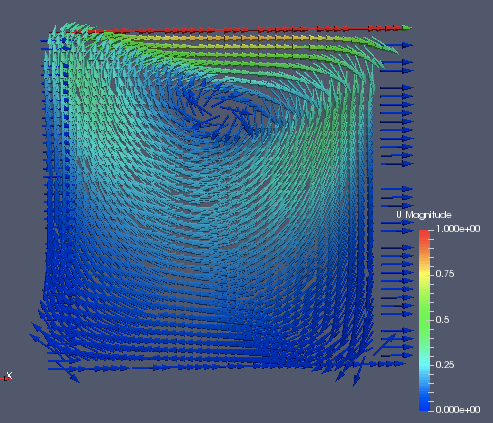
\includegraphics[scale=0.39]{cavity_fine.png}
	\caption{Vectors of cavity case with finer mesh}
	\label{fig:cavity_fine}
\end{figure}

As the mesh has now been refined the details of the vortex can be seen far more clearly. This is, perhaps, not the most useful for this case however when using more complex geometry smaller flow features may be created and if the mesh is not sufficiently fine, the features may be lost. 
//
When studying fluid flow, most of the interesting flow features occur at the wall with the flow becoming less interesting as the distance from the wall increases. To conserve processing power it therefore beneficial to introduce a mesh grading. This is having a finer mesh at the wall with the mesh becoming more coarse as we move away from the wall. 
/
To do this in OpenFOAM in this case the cavity is split into 4 blocks. Additional vertices are created in the mesh file to define the blocks. The mesh for each block is defined. For this case simple grading is introduced. For each block the mesh is defined to be twice as fine at the wall compared to the other end of the block. The number of cells has been reduced with this grading.
\
Due to the change in the cell size the Courant number will change as seen from equation \ref{eq:courant}. The smallest cell size must then be computed then the timestep changed to ensure the Courant number remains below 1. 
\\
To further reduce computational expense the results of the previous simulation can be mapped to the new mesh and the simulation time can be started from this point. The graded mesh is shown in figure \ref{fig:cavity_graded}.  

\begin{figure}[h]
	\centering
	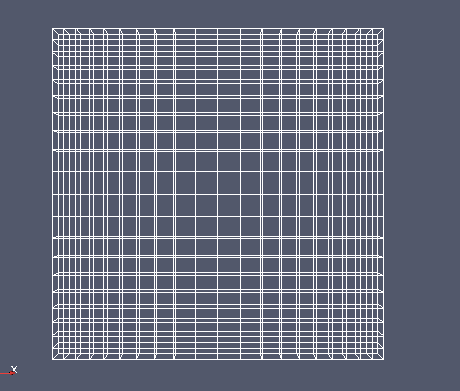
\includegraphics[scale=0.5]{Graded_mesh.png}
	\caption{Graded Mesh For Cavity Case}
	\label{fig:cavity_graded}
\end{figure}

It is clearly seen that the mesh is far finer at the walls compared to the centre of the cavity.
\\
The Reynolds number is then increased an order of magnitude. This is achieved by reducing the kinematic viscosity $\nu$ by a factor of 10. This is clear by the equation for Reynolds number.
\begin{equation}
Re = \frac{UL}{\nu}
\label{eq:reynolds}
\end{equation}
Where $U$ is the flow speed and $L$ is the characteristic length.
 \
 Due to the increase in Reynolds number the overall simulation time is increased. As the Reynolds number is increased the flow changes regime from laminar to turbulent. This means that the variations in flow velocity will be very high hence the mesh will need to be very fine. This is impractical hence Reynolds averaged turbulence models will need to be used. The turbulence models calculate the mean flow behaviour and the random fluctuations. For this case the $k-\epsilon$ model will be used for a Reynolds number of $10^4$.
 \\

The second OpenFOAM tutorial looked at the stress analysis of a plate with a hole. This was thought to be useful as the project will be looking at the structural effects as well as fluid flow.\\

This case was a simple linear-elastic steady state case with the geometry shown in figure \ref{fig:stress_geometry}

\begin{figure}[h]
	\centering
	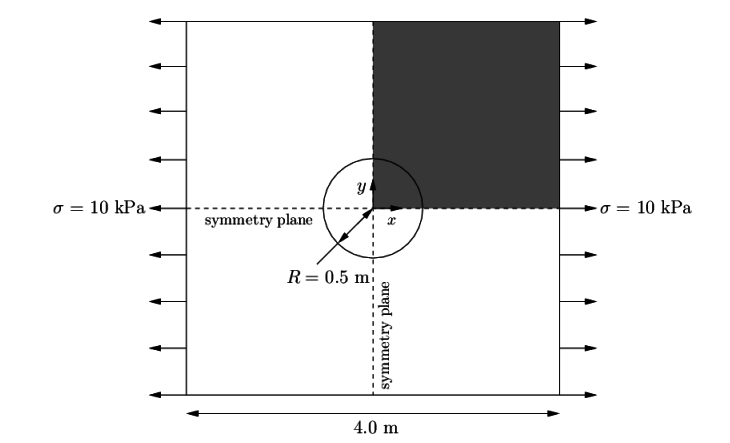
\includegraphics[scale=0.5]{stress_geometry}
	\caption{Geometry for stress analysis case}
	\label{fig:stress_geometry}
\end{figure}

Note there are two lines of symmetry here hence only one quarter of the object need be modelled. The mesh for this is created in a similar way to the cavity case. However for this case there are curved edges. This is accounted for by having 5 blocks with vertices at corners between blocks and the midpoint of the curved edges as shown in figure \ref{fig:stress_cell_def}

\begin{figure}[h]
	
	\begin{minipage}[h]{0.5\textwidth}
		\centering
	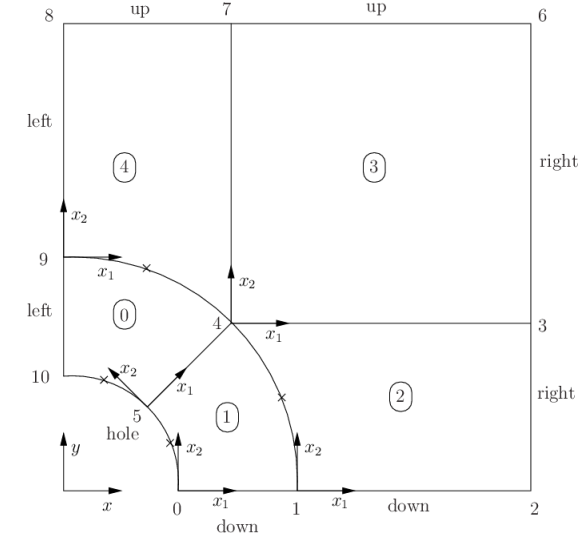
\includegraphics[width = \textwidth]{stress_blocks}
	\caption{Block and Vertex definitions.}
	\label{fig:stress_cell_def}
	\end{minipage}
	\begin{minipage}[h]{0.5\textwidth}
		\centering
	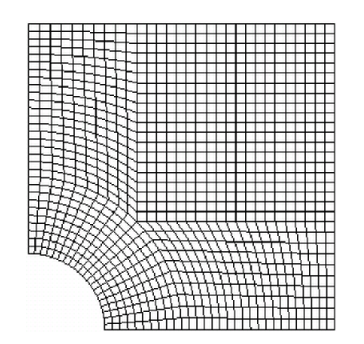
\includegraphics[width = \textwidth]{stress_mesh}
	\caption{Mesh for stress case}
	\label{fig:stress_mesh}
	\end{minipage}
\end{figure}

The curved cells are created using the keyword $edges$ in the mesh generation file. The edges between the vertices which define the curve set to $arc$. In this file the down and left faces are set to symmetry planes to reflect the geometry of the entire plate. This creates the mesh as shown in figure \ref{fig:stress_mesh}
\\
The mechanical properties of the system can then be defined such as density $\rho$, Youngs modulus $E$ and Poissons ratio $\nu$

The code is then run using solidDisplacementFoam. The stress field over the plate can then be viewed using paraview this can be seen in figure \ref{fig:stress_field}

\begin{figure}
	\centering
	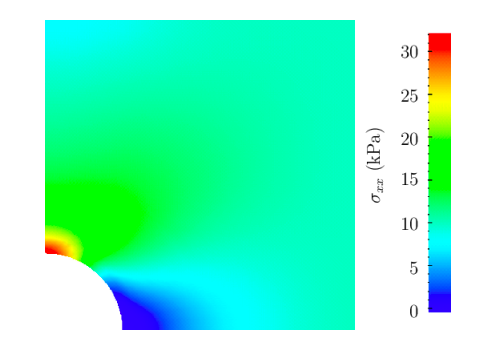
\includegraphics[scale=0.5]{stress_field}
	\caption{Stress field on plate}
	\label{fig:stress_field}
\end{figure}

It can be seen that there is a stress concentration at the top of the hole with decreased stress at the side. This is because the stress through the plate acts like a fluid and is deflected around the hole. 

It is also desirable to compare the numerical results to the analytical solution. This done through OpenFOAM by using a $singleGraph$ file.
The results are then compared and shown on figure \ref{fig:stress_analytical} 

\begin{figure}
	\centering
	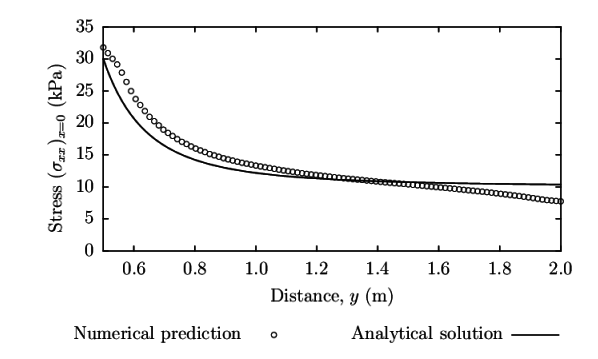
\includegraphics[scale=0.5]{stress_analytical}
	\caption{Analytical Solution compared to numerical solution}
	\label{fig:stress_analytical}
\end{figure}

As seen in figure \ref{fig:stress_analytical} the numerical solution slightly underestimates the stress at the edge of the plate and overestimated the stress at the hole. This can be improved by introducing a finer grid or having mesh grading as described earlier in this chapter


\chapter{Background Theory}
This chapter describes the background theory used to describe the performance of the propeller. *MORE STUFF
\section{Blade Element Momentum Theory}

Blade Element Momentum Theory (BEMT) is a combination of two theories: axial momentum theory and blade element theory. BEMT takes in various geometric parameters such as pitch, chord and camber to produce a body force model of thrust and torque. BEMT also uses various empirical correction factors to correct for tip losses, curvature and wake losses. This section will discuss the theory and solution procedure of BEMT.

\subsection{Momentum Theory}

\begin{figure}
	\centering
	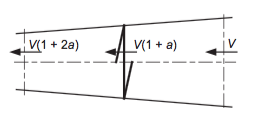
\includegraphics[scale=0.5]{Momentum_theory}
	\caption{Momentum theory}
	\label{fig:momentum_theory}
\end{figure}

Momentum theory is based on the a streamtube with an actuator disc. The actuator disc is an infinitesimally thin disc with an increase in axial velocity occurring at the disc. The axial velocity at the disc is therefore:

\begin{equation}
V_1 = V(1+a)
\end{equation}

Where $a$ is the axial inflow factor and $V$ is the inflow velocity. The axial velocity far downstream is $V_2 = V(1+2a)$. Similar results can be shown for the angular velocity where the angular velocity relative to the blades at the disc is $\Omega (1-a')$ where $\Omega$ is the angular velocity of the disc and $a'$ is the circumferential inflow factor.

The actuator disc as radius $r$ and thickness $\delta r$. The thrust on the disc is therefore:

\begin{equation}
\delta T = 2\pi r \delta r \rho V(1 + a)(V_2 - V)
\label{eq:Thrust_momentum}
\end{equation}

This is the rate of momentum change. Similarly the torque is given by:

\begin{equation}
\delta Q = 2\pi r \delta r \rho V(1 + a)r^2 2 a' \Omega
\label{eq:Torque_momentum}
\end{equation}
Hence the thrust per unit span is given by:

\begin{equation}
\frac{dT}{dr} = 4 \pi r V^2 a (1 + a)
\label{eq:Thrust_unit_span_momentum}
\end{equation}
With Torque given as:
\begin{equation}
\frac{dQ}{dr} = 4 \pi r^3 V \Omega a' (1 + a)
\label{eq:Torque_unit_span_momentum}
\end{equation}

A real propeller is not a disc but a finite number of blades.There must be a correction for this as the flow conditions are not circumferentially uniform (TURNOCK). The Goldstein factor, $K$ (GOLDSTIEN) is introduced into equations \ref{eq:Thrust_unit_span_momentum} and \ref{eq:Torque_unit_span_momentum}. The thrust and torque per unit span are now defined in equations \ref{eq:Thrust_unit_span_goldstein_momentum} and \ref{eq:Torque_unit_span_goldstein_momentum}:

\begin{equation}
\frac{dT}{dr} = 4 \pi r V^2 K a (1 + a)
\label{eq:Thrust_unit_span_goldstein_momentum}
\end{equation}

\begin{equation}
\frac{dQ}{dr} = 4 \pi r^3 V \Omega K a' (1 + a)
\label{eq:Torque_unit_span_goldstein_momentum}
\end{equation}

where $K$ is the Goldstein factor. Charts have been created for propellers with 2-7 blades. However a functional relationship for the correction factor is given by: 
\begin{equation}
K = \frac{2}{\pi} \cos^{-1}(\frac{\cosh(xF)}{\cosh(F)})
\end{equation} 

where $F = \frac{Z}{2x \tan \phi} -\frac{1}{2}$ $Z$ is the number of blades and $\phi$ is the hydrodynamic pitch angle.
\\
The blade element equations are based on figure \ref{fig:blade_element}

\begin{figure}
	\centering
	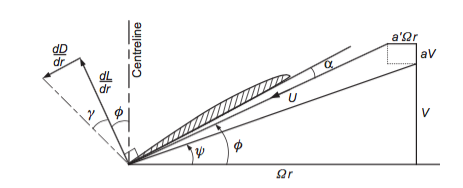
\includegraphics[scale=0.5]{blade_element}
	\caption{Blade element diagram}
	\label{fig:blade_element}
\end{figure}

Where $C_l$ is the lift coefficient and $C_d$ is the drag coefficient which are both dependent on angle of attack $\alpha$. For a two dimensional blade section the lift and drag forces are defined by:

 \begin{equation}
 \frac{dL}{dr} = \frac{1}{2} \rho Z c U^2 C_l
 \label{eq:lift_unit_span}
 \end{equation}
 
  \begin{equation}
 \frac{dD}{dr} = \frac{1}{2} \rho Z c U^2 C_d
 \label{eq:drag_unit_span}
 \end{equation}
 
 The lift and drag can then be resolved in terms of the hydrodynamic pitch angle to give the section thrust and torque. These can then combined with the equations \ref{eq:lift_unit_span} and \ref{eq:drag_unit_span} to give the thrust and torque coefficients: 
\begin{equation}
\frac{dK_T}{dx} = \frac{\pi^2}{4} (\frac{Z_c}{D}) C_L x^2 (1 - a')^2 \sec\phi (1 - \tan \phi \tan \gamma)
\label{eq:Kt/dx}
\end{equation} 

\begin{equation}
\frac{dK_Q}{dx} = \frac{\pi^2}{8} (\frac{Z_c}{D}) C_L x^3 (1 - a')^2 \sec\phi (\tan \phi + \tan \gamma)
\label{eq:KQ/dx}
\end{equation} 
 where $\tan \gamma = \frac{C_D}{C_L}$. Local efficiency $\eta$ can be defined by $\eta = \frac{\tan\psi }{\tan (\phi + \gamma)}$. Which can then be used to compute the inflow factors $a$ and $a'$ through the ideal efficiency $\eta_i = \frac{\tan \psi}{\tan \phi}$. The required lift and drag coefficient can then be computed using equations \ref{eq:Kt/dx} and \ref{eq:KQ/dx}, with the torque coefficient calculated from equation \ref{eq:Thrust_unit_span_goldstein_momentum}.
 
 The flow diagram for the solution procedure is shown in \ref{fig:blade_element_flow_diagram}. In this procedure the advance ratio, pitch/diameter, position along blade and drag coefficient are given. The hydrodynamic pitch angle $\phi$ plus angle of attack $\alpha$ are computed. A first guess of $\alpha$ is then made to calculate $\phi$ which is used to calculate the ideal efficiency. The axial inflow factor $a$ is then computed along with the Goldstein correction factor. In the first case the efficiency $\eta$ is assumed to be equal to the ideal efficiency. The torque coefficient is then calculated as is the lift and drag coefficients which are used to calculate the local efficiency. This value of local efficiency is then used to compute the new axial inflow factor. The procedure is repeated until the local efficiency converges to a value.
 
Once the local efficiency value has converged the required lift coefficient is computed along with the curvature correction. The angle of attack is then calculated from the lift curve slope $\frac{dC_l}{d \alpha}$ and the required lift coefficient. The entire process is repeated until the angle of attack converges. Once $\alpha$ converges the process is repeated at the next position on the blade. This procedure is used in the code described in CHAPTER BLAH! 
 
 \begin{figure}[h]
	\centering
	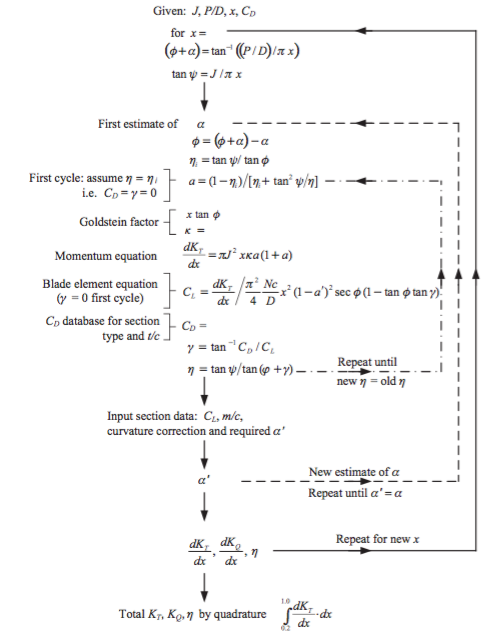
\includegraphics[scale=0.5]{BEMT_flow_diagram}
	\caption{Blade element momentum theory solution procedure flow diagram (TURNOCK)}
	\label{fig:blade_element_flow_diagram}
 \end{figure}
 
As the flow moves along the blade it experiences a change in angular inflow factor. This is taken into account by the addition of curvature correction. The curvature correction is calculated using the Ludweig-Ginzel corrections (REFERENCES). The curvature correction works by firstly approximating $\frac{dC_L}{d(m/c)}$. The camber required to produce the same $C_L$ with 2D flow $\frac{m_0}{c}$ is given by $\frac{m_0}{c} = \frac{C_L}{\frac{dC_L}{d(m/c)}}$ . Therefore:

\begin{equation}
\frac{m}{c} = \frac{m_0}{c} k_1 k_2
\label{eq:m_c}
\end{equation}

Where $k_1$ and $k_2$ are given by the curves shown in figure \ref{fig:curvature_correction_curves}. From this data and the angle of attack a change of lift coefficient can be computed which is used to compute the change camber.
\begin{figure}[h]
	\centering
	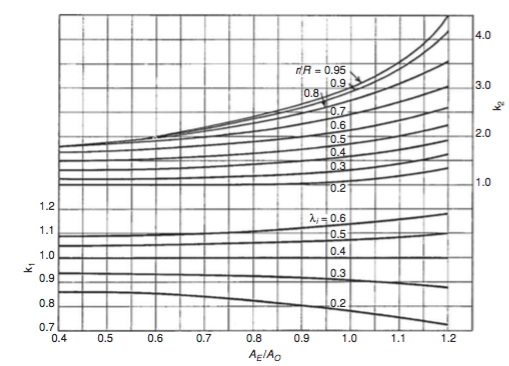
\includegraphics[scale=0.5]{curvature_correction_curves}
	\caption{Ludweig-Ginzel camber correction coefficients (REF) }
	\label{fig:curvature_correction_curves}	
\end{figure}
\newpage
 \section{Timeshenko Beam Theory and Finite Element Analysis}
 
 This section will discuss the theory behind Timoshenko beam theory and finite element analysis. 
 \subsection{Timoshenko Beam Theory}
 Timoshenko beam theory was developed by Stephan Timoshenko in the early 20th century(CITATION). It is used as a model of structural deformation and accounts for shear deformation and rotational effects (BROWN CITE). Because of this it can be used for short thick beams which is useful when studying marine propellers.
 
 \begin{figure}
	\centering
	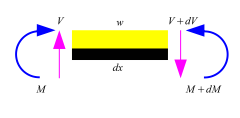
\includegraphics[scale=0.75]{forces_on_beam}
	\caption{Forces on beam}
	\label{fig:forces_on_beam}	
 \end{figure}
 
 Figure \ref{fig:forces_on_beam} shows the forces acting on a beam segment. Here $V$ is the shear force, $M$is the bending moment acting on the beam, $w$ is the load and $dx$ is the section length. 
\
If the equilibrium state is now considered it can be shown:
\begin{equation}
	\sum M_z = 0 = (M+dM) - M - Vdx + W dx \frac{dx}{2}
	\label{eq:equilibrium of moments}
\end{equation}
\begin{equation}
\sum F_y = 0 = V - (V+dV) - W dx
\label{eq:equilibrium of forces}
\end{equation}

It can therefore be shown:
\begin{equation}
w = -\frac{dV}{dx}
\label{eq:Moments}
\end{equation}
and 
\begin{equation}
V = \frac{dM}{dx}
\label{eq:Forces}
\end{equation}
When under a load the beam bends with a radius of deflected curve $\rho$. The curvature is given by $\kappa = \frac{1}{\rho} = \frac{M}{EI}$ where $E$ is the modulus of elasticity and I is the moment of inertia. The beam curves by angle $\phi$ with translational movement $v$ at position $x$ however when the angles are small $\phi = \frac{dV}{dx}$. From figure \ref{fig:curvature} it can be seen that $\kappa = \frac{d^2 v}{d x^2}$.
Hence equating $ \kappa$ gives:
\begin{equation}
M = EI  \frac{d^2 v}{d x^2}
\label{eq:moment EI}
\end{equation}

Substituting equation \ref{eq:Forces} into equation \ref{eq:Moments} and then substituting equation \ref{eq:moment EI} into equation the resulting equation gives:

\begin{equation}
w =- EI  \frac{d^4 v}{d x^4}
\label{eq:load_shear}
\end{equation}

The shears can now be related to the translational displacement by: 
\begin{equation}
V = EI  \frac{d^3 v}{d x^3}
\label{eq:shear_displacement}
\end{equation}


\begin{figure}
	\centering
	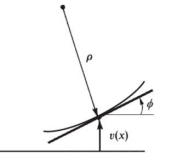
\includegraphics[scale=0.5]{curvature}
	\caption{Curvature on beam at position x}
	\label{fig:curvature}
\end{figure}
 
 
The stress $\sigma$ and strain $\epsilon$ can now be introduced. The displacement in the x-direction is given by $u = -y \theta$
 
 The strain components are therefore: 
 \begin{equation}
\epsilon_{xx} = -y \theta ^{'}
\hspace{5 mm}
\epsilon_{yy} = 0
\label{eq:strain}
\hspace{5 mm}
\gamma_{xy} = -\theta + v^{'}
 \end{equation}
 and the stress is:
  \begin{equation}
 \sigma_{xx} = -E y \theta ^{'}
 \hspace{5 mm}
 \sigma_{yy} = -E \frac{\nu}{1 - \nu ^2} y \theta
 \label{eq:stress}
 \hspace{5 mm}
 \sigma_{xy} = \kappa G \gamma_{xy}
 \end{equation}
 
 The potential energy of the beam is the stored elastic energy plus the energy applied to the beam:
 
 \begin{equation}
 \pi = \frac{1}{2} \int \sigma_{xx} \epsilon_{xx} dV + \frac{1}{2} \int \sigma_{xy} \epsilon_{xy} dV  - \int w v dx
 \label{eq:potential_energy_beam}
 \end{equation}
 When substituting values for strain and stress into equation \ref{eq:potential_energy_beam} the potential energy becomes:
 
  
 \begin{equation}
 \pi = \frac{1}{2} E I  \int_{0}^{L} {\theta '}^2 dx + \frac{1}{2} \kappa G A  \int_{0}^{L} (-\theta + v')^2  dx  -  \int_{0}^{L} w v dx
 \label{eq:potential_energy_beam_sub}
 \end{equation}
 
 and the change in potential energy is:
  \begin{equation}
 \delta \pi =  E I  \int_{0}^{L} \frac{d{\theta}}{dx} \frac{d\delta {\theta}}{dx}dx +  \kappa G A  \int_{0}^{L} (-\theta + \frac{dv}{dx})(\delta \theta - \frac{d \delta v}{dx})  dx  -  \int_{0}^{L} w \delta v dx = 0
 \label{eq:change_in_potential_energy_beam_sub}
 \end{equation}
 
 We now have a system of equations of the form:
 \begin{equation}
 [K]\vec{u} = \vec{F}
 \end{equation}
 Where $K$ is the stiffness matrix, $\vec{u}$ is the displacement vector and $\vec{F}$ is the force vector. There is now a system of equations which describe the beam deformation for a given load. However not all terms in equation \ref{eq:change_in_potential_energy_beam_sub} are known. Approximations must be made for the interpolation of bending $v$ and twist $\theta$. This is done using shape functions. This process is described in section \ref{sec:FEA}.
 
 \subsection{Finite Element Analysis}
 \label{sec:FEA}
 
 Finite element analysis is used to obtain an approximation to properties of structures. The domain is split into many intervals or elements. The governing equation of the property is known however there are terms in the equation which are unknown. These terms are represented using shape functions such that:

 \begin{equation}	
	 \begin{aligned}
	 v = \sum_{a} N^a v^a \hspace{5mm}  \theta = \sum_{a} N^a \theta^a \\
	  \delta v = \sum_{b} N^b \delta v^a \hspace{5mm}  \delta \theta = \sum_{b} N^b \delta \theta^b  
	  \end{aligned}
	  \label{bend_twist shape functions}
 \end{equation} 
The shape functions are chosen such that $N^a = 1$ at the associated node and $N^a = 0$ at all other nodes. For simplicity the shape functions have been chosen to be linear. For this case the shape functions are:

\begin{equation}
N^a = 0.5(1-x_i)
\hspace{5mm}	
N^b = 0.5(1+x_i)
\label{eq:shape functions}
\end{equation}
Where $x_i$ is the local coordinate. From convention $x_i$ is in the interval $[-1,1]$. Equations \ref{bend_twist shape functions} can now be substituted into equation \ref{eq:change_in_potential_energy_beam_sub} to give:

\begin{equation}
\left \{ E I \int_{0}^{L} \frac{d{N^a }}{dx} \frac{d N^b }{dx}dx \right \} w^a  + \left \{ \ - \kappa G A \int_{0}^{L} N^a \frac{d N^b }{dx}dx \right \} \theta^a = \int_{0}^{L} w N^b dx
\label{eq:shape func governing equ}
\end{equation}

This generates the local stiffness matrix and force vector. The local values must then be mapped on to the global stiffness matrix and global force vector. This is relatively simple for a 1D beam.

Equation \ref{eq:shape func governing equ} is now in a form which is solvable via $\vec{u} = \vec{F} [K]^{-1} $. This is done by the code described in section (CODE SECTION HERE)

\chapter{The Code}
\label{ch:code}
This chapter will describe the code used for the blade element momentum theory and finite element analysis. Furthermore the chapter will describe how the BEMT and FEA are coupled. Full code can be found in appendix (INSERT APPENDIX REF)

\section{Blade Element momentum theory code}
The blade element momentum theory code uses the same algorithm as described in figure \ref{fig:blade_element_flow_diagram}. However there are portions which require user input. This section will describe the code and the required user input.

The 1st part of the user needs to interact is the initializing data

\begin{lstlisting}[language = Python]
if __name__ == '__main__':
	Re = 500000 # Reynolds Number
	foil_filename = 'naca2412.dat'
	prop_data_file = 'propgeom.txt'
	P_D = 1.2     # Pitch/Diamter Ratio
	BA_ratio = 0.95 #  Blade Area Ratio
	N_blades = 3    # number of blades
	xfoil_flag = 0 # use xfoil for Cl and Cd approximations 1 yes, 0 no
	rho = 1029 # density of seawater
	n = 10 # rotations per sec
	Va = 10 # prop inflow velocity
	chord, x_R_list, local_P_D, chord_diameter, thickness_distibution,MC,filename \\
	 ,D = generate_foil_data(prop_data_file)
	J = Va/(n*D)   #Advance Ratio
	E = 5e6 # Elastic Modulus
	nu = 0.3 # Poissons Ratio
	kappa = 5/6 
	h = 2 
\end{lstlisting}

Here the basic conditions are defined such as Reynolds number, Elastic modulus and Poissons ratio. Furthermore on line 3 the foil filename is defined. This is the data file defining the foil coordinates. This file is used only if Xfoil is being used to generate the foils lift and drag curves. The option to use Xfoil is specified in line 8, if 1 is selected the Xfoil will be used, if 0 is selected then the lift and drag curves will be defined by a data from a lookup table. \
The propeller data file is defined in line 4. An example of this data file is shown in figure \ref{fig:prop dat file}. This file gives information on the number of blades, section profile,and propeller diameter. The radial positions to be analysed are given as well as: the pitch, chord, camber and thickness at these positions. All this data is stored and used in blade element momentum theory. 
\\
Once the blade parameters have been defined the blade element momentum theory is then called.



\begin{figure}
	\centering
	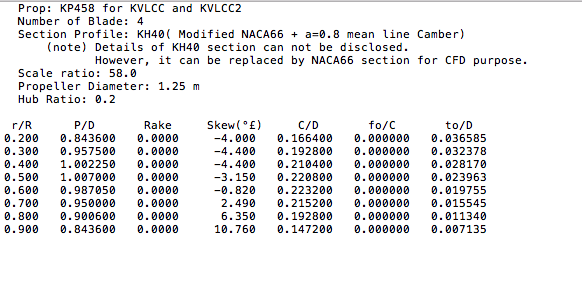
\includegraphics[scale=0.5]{prop_data_file_example}
	\caption{Example of a propeller data file}
	\label{fig:prop dat file}
\end{figure}
Firstly the angle of attack is set to 0 for the 1st blade element.

\begin{lstlisting}[language = Python]
alpha[i] = 0.0
# set number of alpha iterations to 0
alpha_iterations = 0
# set convergence flag to 0
alpha_converge = 0
# start of alpha convergenc loop
while alpha_iterations < 2000 and alpha_converge == 0: 
	alpha_iterations += 1
	# calculate tan of inflow angle
	tan_psi[i] = J / (np.pi*x_R)
	# induced flow angle plus angle of attack
	phi_plus_alhpa[i] = np.arctan2(local_P_D[i],(np.pi*x_R))
	# inflow angle
	phi[i] = phi_plus_alhpa[i] - alpha[i]
	# ideal efficieny
	eta_ideal = tan_psi[i] / np.tan(phi[i])
	# initially set efficiency to ideal  
	eta  = 0.9 * eta_ideal
	gamma = 0.0 # zero for ideal efficiency
\end{lstlisting}
The alpha loop then begins. Firstly the inflow angle is calculated from the advance ratio. Then the induced flow angle plus angle of attack is computed from the local pitch (line 12). The angle of attack is then subtracted from this to compute the induced flow angle. The ideal efficiency is then calculated from the inflow angle and induced flow angle and the actual efficiency is set to 90\% of the ideal efficiency.
\\
The efficiency loop now begins.
\begin{lstlisting}
while eta_iterations < 2000 and eta_converge == 0:
	# axial inflow factor
	a = (1 - eta_ideal)/(eta_ideal + (tan_psi[i]**2)/eta)
	# local thrust coefficient
	KT_dx[i] = np.pi*(J**2) * x_R * K * a*(1+a)
	# circumferential inflow factor (a')
	a_p =1-eta_ideal*(1+a)
\end{lstlisting}
Firstly the axial and circumferential inflow factors are computed as shown in lines 3 and 7. The thrust coefficient is also computed. The lift and drag coefficients are then computed. This is done using a table either produced by Xfoil or using the look up table. The table has values for lift and drag coefficient for many angles of attack. If the angle of attack of the blade section does not lie on a defined value simple linear interpolation is used. A new $\gamma$ angle is calculated from the lift and drag coefficients. From the new $\gamma$ the efficiency is computed. This efficiency loop is then repeated until $\eta_{old} = \eta_{new}$ within a small tolerance.
\\
Once the efficiency has converged the curvature correction is applied. This involves generating correct coefficients $k_1$ and $k_2$ using the graph shown on figure \ref{fig:curvature_correction_curves}. The rate of change of lift coefficient to camber is assumed to be 12 (TURNOCK). The camber deficit is then computed by subtracting the required camber at $\alpha = 0$ from the actual camber. This is then multiplied by the assumed lift coefficient camber slope and divided by the lift curve slope to produce the new angle of attack. This process is repeated until the angle of attack converges on a single value. 
\ 
When the angle of attack converges the torque coefficient is calculated as is the velocity of the fluid into the blade element. The entire process is repeated for the next blade element. 
\\
Once the process is complete over all blade elements the total thrust and torque coefficients are computed by integrating the thrust and torque over all elements using Simpsons rule. The results of this process are shown in chapter \ref{ch:Results and Discussion}.

\section{Finite Element Analysis Code}
The model of the blade for structural purposes is that of a simple 1D timoshenko beam. This makes the computational cost of computing the bending and twist cheap whilst also having good accuracy. 
\\
The code starts by creating a grid of nodes evenly spaced along the beam. The number of nodes is defined by the number of elements. A location matrix is then set up to define the global node numbers to define each element. In other words, the nodes defining each element 1 will be stored in column 1 in the location matrix. An example of the location matrix  is shown in matrix \ref{eq:location matrix}
\begin{equation}
LM = 
 \left[ \begin{array}{ccccccc}
 	\centering
0 &1 &2 &3& 4& 5& 6\\
	1& 2& 3& 4& 5& 6& 7 
\end{array}\right]
\label{eq:location matrix}
\end{equation}

The integration points on each element are then defined. The integration will be an Gaussian quadrature. Therefore, for ease of calculation the weighting will be set to 1 hence the integration points chosen are $\pm \sqrt{\frac{1}{3}}$. For more on Gaussian quadrature see Appendix B.
\
So for each element and each integration point of each element the value of the shape functions described in equations \ref{eq:shape functions} are computed. The shape function derivatives are with respect to local coordinates so therefore must be converted to global coordinates this is done using the chain rule.\
The stiffness matrix contributions due to bending are computed 1st with the global stiffness matrix and global force vector being populated appropriately as consistent with equation \ref{eq:shape func governing equ}. \
Note that np.meshgrid is being used here. This is to ensure that the correct elements of the stiffness matrix are being populated. np.meshgrid creates matrix from the two arrays it is given. This matrix allows a every combination of element pairs in the row and columns. It is therefore used in the stiffness matrix population to populate every element in the matrix which corresponds to the bending and twist of the finite element.
\\
The shear contribution is then added to the global stiffness matrix. This process is repeated for every element over the entire beam.
\ The boundary conditions are then enforced. For this case the propeller blade is treated as a cantilever beam. This means that the bending and rotation at base are strictly zero. This boundary condition is set and the system of equations $\vec{u} = \vec{F}[K]^{-1}$ is solved to give the bending and twist along the beam.

\section{Interface between blade element momentum theory and finite element analysis}
There is now a function which returns the thrust and torque, and another function which computes the bending and twist of a beam for a given load. It is desirable to combine the two pieces of code. This section describes how the two codes are combined.

The blade element momentum theory code returns the thrust,torque, flow speed at each element and the lift coefficient. The lift force can then be computed by the formula \ref{eq:lift equation}

\begin{equation}
 L = \frac{1}{2} \rho U^2 S C_L
 \label{eq:lift equation}
\end{equation} 

Where $\rho$ is the fluid density, $U$ is the flow speed, $S$ is the surface area and $C_L$ is the lift coefficient. The lift force can then be calculated for each element. This is the force which acts perpendicular to the blade as shown in figure \ref{fig:blade_element} so will be used as the load on the Timoshenko beam. 
\
The main difficulty of combining the blade elements to the finite elements is mapping the loads to the correct elements. The code has been written such that the number of finite elements is independent to the number of blade elements. This therefore requires additional code to map the blade element loads to the finite elements. This code is shown below.

\begin{lstlisting}
def BEMT_FEA_mesh_interp(N_elements_FEA,N_elements_BEMT,Cl,L):
	LM_BEMT = np.zeros((2,N_elements_BEMT))
	LM_FEA = np.zeros((2,N_elements_FEA))
	for e in range(N_elements_BEMT):
		LM_BEMT[0,e] = e*L/N_elements_BEMT
		LM_BEMT[1,e] = (e+1)*L/N_elements_BEMT
	
	for e in range(N_elements_FEA):
		LM_FEA[0,e] = e*L/N_elements_FEA
		LM_FEA[1,e] = (e+1)*L/N_elements_FEA
	
	q = np.zeros(N_elements_FEA)
	residual = 0
	for j in range(N_elements_FEA):   
		k = j 
		for i in range(N_elements_BEMT):
			if LM_FEA[0,k] >= LM_BEMT[0,i] and LM_FEA[1,k] <= LM_BEMT[1,i]:
				q[k] = Cl[i]
				k+=1
			elif LM_FEA[0,k] < LM_BEMT[1,i] and LM_FEA[1,k] > LM_BEMT[1,i]:
				residual = abs(LM_FEA[1,j] - LM_BEMT[1,i])
				q[k] = residual*Cl[i] + (1-residual)*Cl[i+1]
				k+=1
	return q
\end{lstlisting}

From the code above two location matrices are created, one for the blade element momentum theory the other for the finite element analysis. These location matrices are created to define the positions of each node pairs in terms of their global positions on the beam. From line 14 the force is distributed along the finite elements. Line 17 states that if the finite element is within a blade element then set the load on the element equal to the lift force. Line 20-22 states that if the finite element is between two blade elements then the load on the finite element is a combination of the two blade element lift forces and is dependent on how much the finite element breeches the next blade element. This creates a load distribution which is generic for any number of blade elements or finite elements.

\chapter{Results and Discussion}
\label{ch:Results and Discussion}
This section will discuss the results obtained using the code described in chapter \ref{ch:code}. Two test cases have been performed so far. A zero camber case and a  case with camber. From the preliminary investigation the zero camber case works well. However some aspects of the cambered case are wrong.

\section{Zero camber case}

The zero camber case propeller data file is shown in figure \ref{fig:prop dat file}. This is data used on FORTRAN code so can be used for verification. The initial settings are shown in table \ref{tab:zero camber test case}.

\begin{table}[htb]
	
	\label{tab:zero camber test case}
	\centering
	\begin{tabular}{c|l}
		Condition & Value  \\ 	
		\hline
		Advance Ratio $J$ & 0.8 \\
		Blade Area ratio & 0.4 \\
		Number of Blades & 4 \\
		Pitch Diameter ratio & 0.95 \\
	\end{tabular}
\caption{Conditions for zero camber test case.}
\end{table}

The results of the blade element momentum theory are shown in table \ref{tab: zero camber results}. These results match reasonably closely with the results from the FORTRAN code. The difference being the use of a look up table in the code used here as opposed to the analytical approximation used in the FORTRAN code.
\begin{table}[htb]
	\label{tab:zero camber results}
	\centering
	\begin{tabular}{c|l|l}
		 & Python & FORTRAN \\ 	
		\hline
		Thrust Coefficient  & 0.108 & 0.113 \\
		Torque Coefficient & 0.018 & 0.019 \\
		Open water efficiency & 0.737 & 0.746\\
	\end{tabular}
	\caption{Verification of test case using Python and FORTRAN}
\end{table}

Furthermore if the thrust coefficient is plotted against the radial position it can be seen from figure \ref{fig:thrust_position} that the thrust coefficient against radial position is similar to the expected curve shown in figure 15.9 in (TURNOCK) 

\begin{figure}
	\centering
	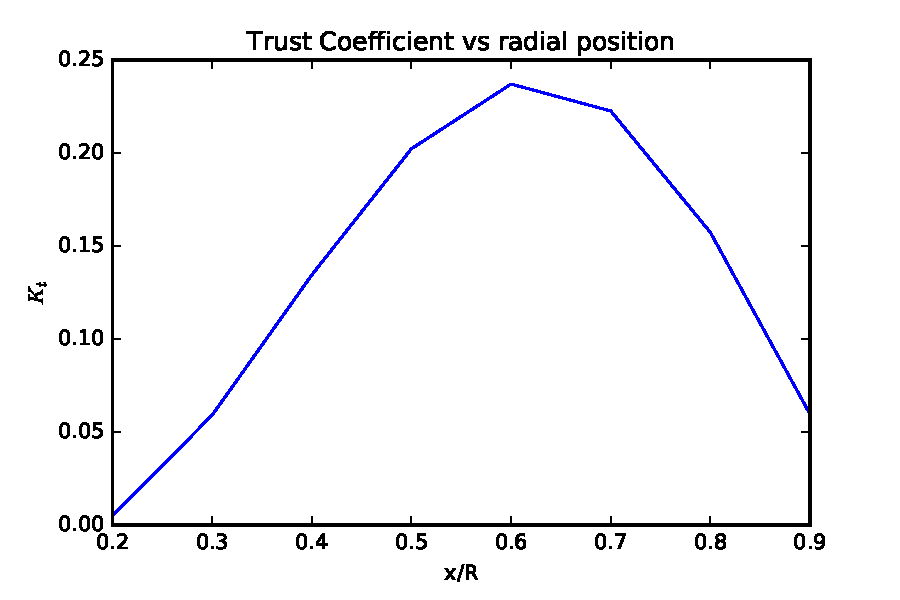
\includegraphics[scale=0.5]{thrust_position.pdf}
	\caption{Thrust coefficient against radial position for the zero camber test case}
	\label{fig:thrust_position}
\end{figure}

This gives a good indicator that the code works well. Given the blade element momentum theory results the finite element analysis is performed. It can be seen from figure \ref{fig:displacement zero camber} that the blade deforms slightly with a maximum deflection at the tip of less than 5mm. 

\begin{figure}
	\centering
	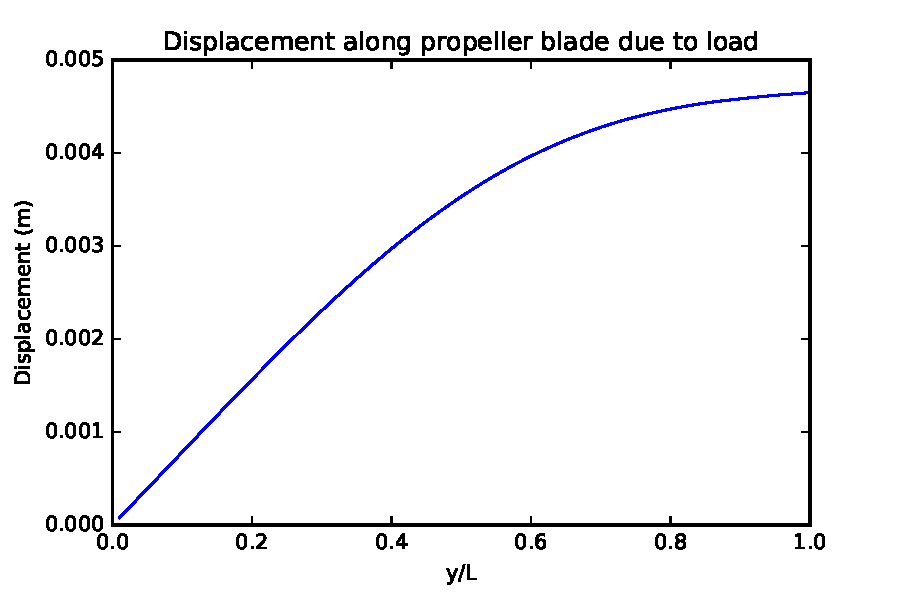
\includegraphics[scale=0.5]{displacement_zero_camber.pdf}
	\caption{Displacement of blade due to loading from lift.}
	\label{fig:displacement zero camber}
\end{figure}
These results seem reasonable however the finite element code must be verified. This is done using another finite element code (BROWN UNI). The verification beam is modelled as a cantilever of length 10m with a uniformly distributed load of 1000N. The distribution deformation matches closely to the expected value as shown in figure \ref{fig:deformation test}
\begin{figure}
	\centering
	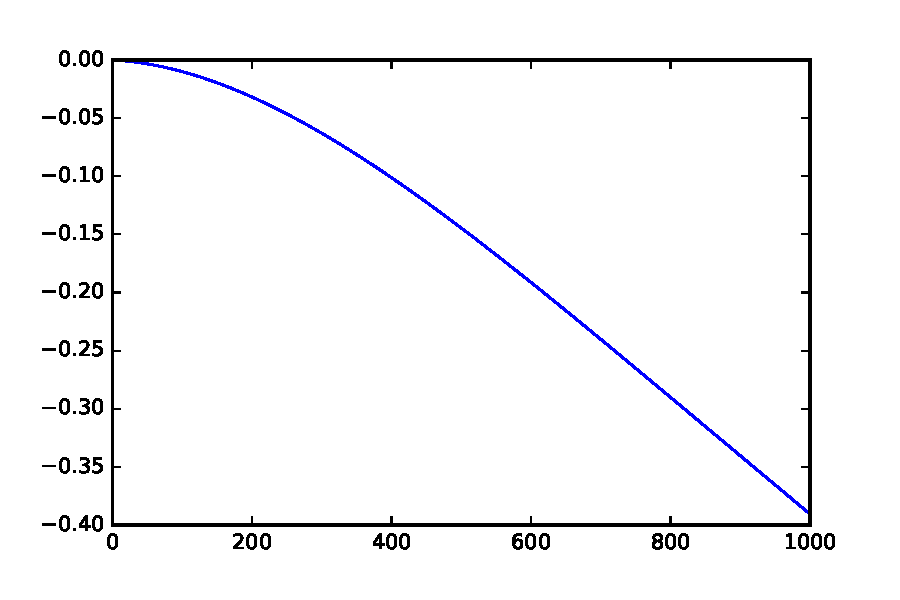
\includegraphics[scale=0.5]{timo_test.pdf}
	\caption{Displacement of test beam due to known loading.}
	\label{fig:deformation test}
\end{figure}

The maximum deformation occurs at element 1000. The deformation is -0.39 m. We can therefore have some confidence that the FEA code gives correct results.

\end{document}          
